\documentclass[UTF8]{article}%z指定文档类型
\usepackage[UTF8]{ctex}%显示中文
\usepackage{graphicx}%引用图包
\usepackage{amsfonts,amsmath,amssymb,amstext}%数学相关宏包
\usepackage{color}

\begin{document}%文章开始


\title{网络通信}%文章题目
\maketitle% 显示上述标题信息

\section{Linux基础知识}

\subsection{linux内核}

内核是操作系统的核心,具有很多最基本功能,它负责管理系统的进程、内存、设备驱动程序、文件和网络系统,决定着系统的性能和稳定性。

Linux 内核由如下几部分组成:内存管理、进程管理、设备驱动程序、文件系统和网络管理等。如图所示:

\begin{figure}[htb!]%插入图片
    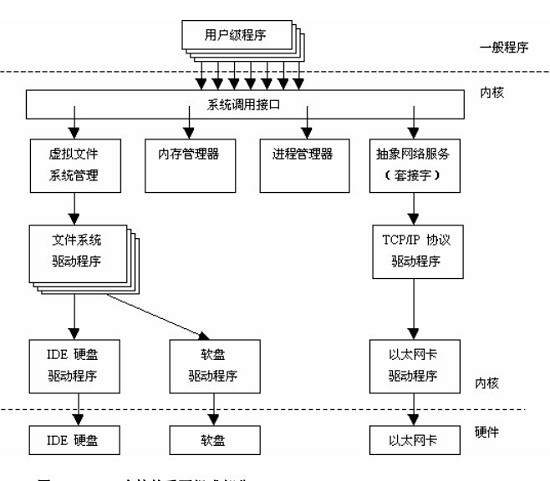
\includegraphics[width=0.8\textwidth]{1.1-1.jpg}
\end{figure}

其中系统调用接口:SCI 层提供了某些机制执行从用户空间到内核的函数调用。

\subsection{Linux 远程登录}

Linux 系统中是通过 ssh 服务实现的远程登录功能,默认 ssh 服务端口号为 22。

安装ssh:yum install ssh

启动ssh:service sshd start

登录远程服务器:ssh -p 50022 my@127.0.0.1

输入密码:my@127.0.0.1:
(-p 后面是端口,my 是服务器用户名,127.0.0.1 是服务器 ip)

回车输入密码即可登录。

\subsection{Linux 进程}

在 Linux 系统中,能够同时运行多个进程,Linux 通过在短的时间间隔内轮流运行这些进程而实现“多任务”。这一短的时间间隔称为“时间片”,让进程轮流运行的方法称为“进程调度” ,完成调度的程序称为调度程序。

Linux 中常见的进程间通讯机制有信号、管道、共享内存、信号量和套接字等。

\subsubsection{相关命令}

可以使用\$ps命令来查询正在运行的进程,比如\$ps -e、-o pid,-o comm,-o cmd,

其中-e表示列出全部进程,-o pid,-o comm,-o cmd分别表示需要PID,COMMAND,CMD信息。

三个信息的意义依次为:PID(process IDentity)是每一个进程的身份(唯一),是一个整数,进程也可以根据PID来识别其他的进程;COMMAND是这个进程的简称;CMD是进程所对应的程序以及运行时所带的参数。

\subsubsection{Linux进程的产生}

当计算机开机的时候,内核(kernel)只建立了一个init进程。Linux内核并不提供直接建立新进程的系统调用。其他所有进程都是init进程通过fork机制建立的。

fork表示:新的进程要通过老的进程复制自身得到,它是一个系统调用。进程存活于内存中。每个进程都在内存中分配有属于自己的一片空间 (address space)。当进程fork的时候,Linux在内存中开辟出一片新的内存空间给新的进程,并将老的进程空间中的内容复制到新的空间中,此后两个进程同时运行。

老进程成为新进程的父进程(parent process),而相应的,新进程就是老的进程的子进程(child process)。一个进程除了有一个PID之外,还会有一个PPID(parent PID)来存储的父进程PID。如果我们循着PPID不断向上追溯的话,总会发现其源头是init进程。所以说,所有的进程也构成一个以init为根的树状结构。

\subsubsection{Linux进程的消失}

当子进程终结时,它会通知父进程,并清空自己所占据的内存,并在内核里留下自己的退出信息(exit code,如果顺利运行,为0;如果有错误或异常状况,为>0的整数)。在这个信息里,会解释该进程为什么退出。

父进程在得知子进程终结时,有责任对该子进程使用wait系统调用。这个wait函数能从内核中取出子进程的退出信息,并清空该信息在内核中所占据的空间。

但是,如果父进程早于子进程终结,子进程就会成为一个孤儿(orphand)进程。孤儿进程会被过继给init进程,init进程也就成了该进程的父进程。init进程负责该子进程终结时调用wait函数。

注意:在Linux中,线程只是一种特殊的进程。多个线程之间可以共享内存空间和IO接口。所以,进程是Linux程序的唯一的实现方式。

\subsection{Linux内存管理}

了让有限的物理内存满足应用程序对内存的大需求量,Linux 采用了称为“虚拟内存”的内存管理方式。Linux 将内存划分为容易处理的“内存页”(对于大部分体系结构来说都是 4KB)。Linux 包括了管理可用内存的方式,以及物理和虚拟映射所使用的硬件机制。

\subsection{Linux文件系统}

Linux系统能支持多种目前流行的文件系统,如EXT2、 EXT3、 FAT、 FAT32、 VFAT和ISO9660。

Linux下面的文件类型主要有:

1) 普通文件:C语言元代码、SHELL脚本、二进制的可执行文件等。分为纯文本和二进制;

2) 目录文件:目录,存储文件的唯一地方;

3) 链接文件:指向同一个文件或目录的的文件;

4) 设备文件:与系统外设相关的,通常在/dev下面。分为块设备和字符设备;

5)管道(FIFO)文件: 提供进程之间通信的一种方式;

6)套接字(socket) 文件: 该文件类型与网络通信有关;

可参考:https://www.linuxprobe.com/linux-system-structure.html

\subsection{Linux防火墙}

\subsubsection{常用命令}

\begin{itemize}
    \item 启动:systemctl start firewalld
    \item 重启:systemctl restart firewalld
    \item 停止:systemctl stop firewalld
    \item 重新加载:firewall-cmd --reload
    \item 查看firewalld的运行状态:
    
        firewall-cmd --state

    \item 取消开放https服务,即禁止https服务:
    
        firewall-cmd --zone=drop --remove-service=https

    \item 开放22端口:
    
        firewall-cmd --zone=drop --add-port=22/tcp

    \item 取消开放22端口:
    
        firewall-cmd --zone=drop --remove-port=22/tcp

    \item 开放两个端口:
    
    firewall-cmd --zone=drop --add-port=8080-8081/tcp

    \item 查询drop区域开放了哪些端口:
    
    firewall-cmd --zone=drop --list-ports

    \item 其他常用命令:
    
    允许icmp协议流量,即允许ping:

    firewall-cmd --zone=drop --add-protocol=icmp

    取消允许icmp协议的流量,即禁ping:

    firewall-cmd --zone=drop --remove-protocol=icmp
    
    查询drop区域开放了哪些协议:

    firewall-cmd --zone=drop --list-protocols

    将原本访问本机888端口的流量转发到本机22端口:
    
    firewall-cmd --zone=drop --add-forward-port
    =port=888:proto=tcp:toport=22
\end{itemize}


\section{socket基础}

\subsection{socket通信的概念}

套接字,运行在计算机中的两个程序通过socket建立起一个通道,数据在通道中传输。套接字可以看成是两个网络应用程序进行通信时,各自通信连接中的端点,这是一个逻辑上的概念。它是网络环境中进程间通信的API(应用程序编程接口)(是IP地址和端口结合)。

socket把复杂的TCP/IP协议族隐藏了起来,只要用好socket相关的函数,就可以完成网络通信。

\subsection{socket的分类}

socket提供了流(stream)和数据报(datagram)两种通信机制,即流socket和数据报socket。

流socket基于TCP协议,是一个有序、可靠、双向字节流的通道,传输数据不会丢失、不会重复、顺序也不会错乱。类似于打电话。

数据报socket基于UDP协议,不需要建立和维持连接,可能会丢失或错乱。UDP不是一个可靠的协议,对数据的长度有限制,但是它的速度比较高。类似于短信。

在实际开发中,数据报socket的应用场景极少。

\subsection{socket通信的过程}

\subsubsection{服务端}

\begin{itemize}
    \item 创建服务端的socket。socket()
    \item 把服务端指定的用于通信的ip地址和端口绑定到socket上。bind()
    \item 把socket设置为监听模式,以监听用户请求。listen()
    \item 接受客户端的连接。accept()
    \item 与客户端通信,接收客户端发过来的报文后,回复处理结果。send()/recv()
    \item 不断的重复上一步步,直到客户端断开连接。
    \item 关闭socket,释放资源。close()
\end{itemize}

\subsubsection{客户端}

\begin{itemize}
    \item 创建客户端的socket。socket()
    \item 向服务器发起连接请求。connect()
    \item 与服务端通信,发送一个报文后等待回复,然后再发下一个报文。send()/recv()
    \item 不断的重复上一步,直到全部的数据被发送完。
    \item 关闭socket,释放资源。close()
\end{itemize}

<<<<<<< HEAD
\subsection{Socket文件描述符}

在Linux系统中,一切输入输出设备皆文件。而socket本质上可以视为一种特殊的文件,即通信的实现,因此socket的通信过程也可以理解为通过“打开open –> 读写write/read –> 关闭close”模式的操作过程。

\subsection{客户端服务端主要参数及结构体}

\subsubsection{socket()返回的值}

返回值称为socket描述符(socket descriptor),其本质是一个文件描述符,是一个整数。把它作为参数,通过它来进行一些读写操作。

\subsubsection{struct hostent* h}

域名和网络地址结构体:

struct hostent

\{

\qquad    char *h\_name;  //主机名,即官方域名
    
\qquad    char **h\_aliases;  //主机所有别名构成的字符串数组,同一IP可绑定多个域名

\qquad    int h\_addrtype; //主机IP地址的类型,例如IPV4(AF\_INET)还是IPV6

\qquad    int h\_length;  //主机IP地址长度,IPV4地址为4,IPV6地址则为16

\qquad    char **h\_addr\_list;  //主机的ip地址,以网络字节序存储。若要打印出这个IP,需要调用inet\_ntoa()。

\};


\subsubsection{struct sockaddr\_in servaddr}

表示地址信息的数据结构(体),存放了目标地址和端口。与结构体sockaddr把目标地址和端口信息混在一起了不同,其把port和addr 分开储存在两个变量中。

struct sockaddr\_in

\{

\qquad sa\_family\_t \quad servaddr.sin\_family; //协议族,在socket编程中只能是AF\_INET。

\qquad unit16\_t \quad servaddr.sin\_addr.port; //16位的TCP/UDP端口号。

\qquad In\_addr\_t \quad servaddr.sin\_addr.s\_addr; //32位IP v4地址。(其中sin\_addr是一个结构体类型变量,表示32位IP地址,内仅包含s\_addr一个变量)

\qquad char \quad sin\_zero[8]; //不使用。

\}

\paragraph{操作函数}~{}

\begin{itemize}
    \item 绑定IP地址:

    servaddr.sin\_addr.s\_addr = inet\_addr("192.168.149.129");  // 指定ip地址

    servaddr.sin\_addr.s\_addr = htonl(INADDR\_ANY);  // 本主机的任意ip地址

    \item 绑定的通信端口:
    
    m\_servaddr.sin\_port = htons(5000);  // 通信端口

    \item 
\end{itemize}

\subsection{客户端服务端函数}

以下为几种常用的接口函数:

\subsubsection{socket()函数}

功能:用于创建一个新的socket。对应于普通文件的打开操作。

返回值:成功则返回一个socket描述符,失败返回-1,错误原因存于errno 中。

使用范围:客户端、服务端。

\paragraph{函数声明}~{}

int socket (int domain, int type, int protocol);

\begin{itemize}
    \item domain:协议域,又称协议族(family)。协议族决定了socket的地址类型,在通信中必须采用对应的地址。
    
        AF\_INET:决定了要用ipv4地址(32位的)与端口号(16位的)的组合;

        AF\_UNIX:决定了要用一个绝对路径名作为地址。

    \item type:指定socket类型。
    
        流式socket(SOCK\_STREAM)是一种面向连接的socket,针对于面向连接的TCP服务应用。数据报式socket(SOCK\_DGRAM)是一种无连接的socket,对应于无连接的UDP服务应用。

    \item protocol:指定协议。
    
        常用协议有IPPROTO\_TCP、IPPROTO\_UDP、IPPROTO\_STCP、IPPROTO\_TIPC等,分别对应TCP传输协议、UDP传输协议、STCP传输协议、TIPC传输协议。

        注意为0则与type相匹配,与type不能随意匹配。

    \item 正常情况,第一个参数只能填AF\_INET,第二个参数只能填SOCK\_STREAM,第三个参数只能填0。
\end{itemize}

使用:int sockfd = socket(AF\_NET,SOCK\_STREAM,0))

\subsubsection{gethostbyname()函数}

功能:把ip地址或域名转换为hostent 结构体表达的地址。

返回值:如果成功,返回一个hostent结构指针,失败返回NULL。

适用范围:客户端。

注意:只要地址格式没错,一般不会返回错误。失败时不会设置errno的值。

\paragraph{函数声明}~{}

struct hostent *gethostbyname(const char *name);

name:域名或者主机名,例如"192.168.1.3"、"www.freecplus.net"等。

使用:struct hostent *h = gethostbyname(argv[1])

\subsubsection{附注:memset()函数}

void *memset(void *str, int c, size\_t n)

str -- 指向要填充的内存块。

c -- 要被设置的值。该值以 int 形式传递,但是函数在填充内存块时是使用该值的无符号字符形式。默认0。

n -- 大小,sizeof(str)。

\subsubsection{connect()函数}

功能:客户端通过调用connect函数来建立客户端socket与服务器的连接。

返回值:成功则返回0,失败返回-1,错误原因存于errno 中。

适用范围:客户端。

注意:如果服务端的地址错了,或端口错了,或服务端没有启动,connect一定会失败。

\paragraph{函数声明}~{}

int connect(int sockfd, const struct sockaddr *addr, socklen\_t addrlen);

sockfd:客户端的socket描述字。

*addr:服务端的socket地址。

addrlen:为服务端socket地址的长度(addr结构体的大小)。

使用:\textcolor{red}{connect(sockfd, (struct sockaddr *)\&servaddr,sizeof(servaddr))}

\subsubsection{bind()函数}

功能:服务端把自身用于通信的地址和端口绑定到socket上。

返回值:成功则返回0,失败返回-1,错误原因存于errno 中。

适用范围:服务端。

注意:如果绑定的地址错误,或端口已被占用,bind函数一定会报错,否则一般不会返回错误。

\paragraph{函数声明}~{}

int bind(int sockfd, const struct sockaddr *addr, socklen\_t addrlen);

sockfd:服务端socket描述字。

*addr:表示服务端的socket地址。一个const struct sockaddr *指针,指向要绑定给sockfd的协议地址。addr。

addrlen:表示服务端addr结构体的大小。

使用:\textcolor{red}{bind(listenfd,(struct sockaddr *)\&servaddr,sizeof(servaddr));}
=======
\subsection{客户端服务端程序概要}

\subsubsection{socket文件描述符}

在Linux系统中,一切输入输出设备皆文件,socket()函数的返回值其本质是一个文件描述符,是一个整数。而socket本质上可以视为一种特殊的文件,即通信的实现,因此socket的通信过程也可以理解为通过“打开open –> 读写write/read –> 关闭close”模式的操作过程。

以下为几种常用的接口函数:

\subsubsection{socket函数}
>>>>>>> 5850692b1d9cac0d894320453843b295c9ff51e5



int socket (int \_domain, int \_type, int \_protocol) \_THROW ;





\begin{itemize}
    \item 
    \item 
    \item 
\end{itemize}

\end{document}%文章结束
